\section{Methodology}
\subsection{data set}
The data set will be used in this project is the Semeion Handwritten Digit Data Set which was obtained from the UCI Machine Learning Repository. The data set consists of 1593 writing samples taken from 80 people. Each participant was told to write two copies of each of the digits zero through nine . One of the copies was supposed to be written as carefully or correctly as possible as shown in Figure \ref{fg:ds1}, while the other copy was to be written as fast as possible, or with errors as shown in Figure \ref{fg:ds2}. Each written digit was then fit into a $16 \times 16$ box, and was represented as a 256 elements array where each element is represented by binary data.\\

\begin{figure}[h]
\centering
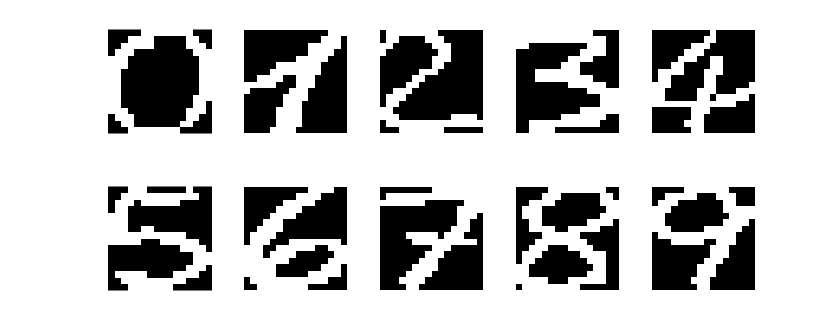
\includegraphics[scale=0.5]{Digits.png}
\caption{Sample digits which written carefully}
\label{fg:ds1}
\end{figure}

\begin{figure}[h]
\centering
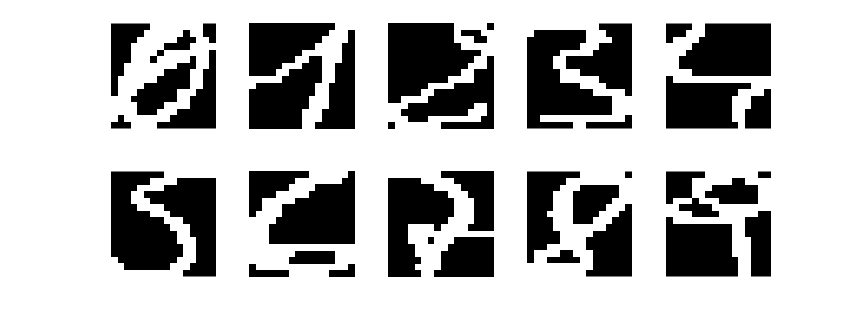
\includegraphics[scale=0.5]{Digits-hnd.png}
\caption{Sample digits which written fast}
\label{fg:ds2}
\end{figure}

\subsection{Experiment Setup}
As mentioned in section 3.1, each handwritten digits was fit into a $16 \times 16$ box, so the hopfield network in this project has 256 neurons. The size of corresponding weight matrix is $256 \times 256$ and all of weights on the diagonal is set to be zero since $w_{ii} = 0$. Also, we will use Hebbian learning rule to train the weights of Hopfield network.\\

Those carefully written digits will be implemented as the training set of Hopfield network. And those digits to be written fast will be used as test cases. Also, Hopfield network requires the data to be $\pm 1$, however the Semeion handwritten data is a 0/1 binary data, so we need to convert the 0/1 binary data to $\pm 1$. \\

In the following experiments, the project will start with storing two memories(digits 0 and 1) to test how well four different sample digits could convergent to the correct stable state. And then will look at the convergence of the same four sample digits with storing three memories (digits 0, 1 and 2), four memories (digits 0, 1, 2 and 3), and finally ten memories (digits 0, 1, 2, 3, 4, 5, 6, 7, 8, and 9). The experiments will show the relationship between the number of memories stored in the network and the capacity of Hopfield network. \\

Finally, this project will try to improve the capacity of Hopfield network by defining an objective function that measures how well the network stores all the memories. I will run through the data set and record the percentage of correct convergences when storing two, three, five, nine and ten digits. This experiment is expected to show the how could we improve the capacity of Hopfield network by modifying its learning rule.
